%!TEX root = ../Sensors_SmartConstruction.tex
% -*- root: ../Sensors_SmartConstruction.tex -*-

\section{Interaction Design}

\subsection{Interacting Method}



제안하는 시스템은 컴퓨팅 인터페이스에 익숙하지 않은 작업 인부들도 직관적으로 3차원 정보에 접근하고 작업을 처리할 수 있도록 하기 위하여 펜과 finger를 사용하여 직관적인 인터페이스를 제공하도록 설계하였다. 이러한 방법은 기존의 3D 모델 처리를 위한 Interactive Tabletop 연구들\cite{brandl_combining_2008, lopes_combining_2011}에서 많이 연구되었으며, 본 논문에서는 이러한 방법을 3차원 공간으로 확장하였다. 특히 \cite{guiard_asymmetric_1987}에서는 양 손의 역할에 대하여 비대칭적인 관계가 있음을 증명하였다. 이에 제안하는 시스템에서도 dominant hand(DH)로 이루어지는 펜 인터렉션과 non-dominant hand(NDH)로 이루어지는 Finger 인터렉션을 구분하여 설계하였다.

%% 번역 원본
% The proposed system was designed to provide intuitive interfaces using a pen and fingers so that workers unaccustomed to computing interfaces can deal with 3D information and manipulate them. This method was studied a lot in interactive tabletop research \cite{brandl_combining_2008, lopes_combining_2011} for the treatment of existing 3D models. In this paper, this method was expanded into 3D space. Especially, in \cite{guiard_asymmetric_1987}, it was proved that there was asymmetric relation about the role of both hands. Hence, in the proposed system, from dividing pen interaction being composed of the dominant hand (DH) and finger interaction being composed of the non-dominant hand (NDH), the design was conducted.

%% 번역 결과
% The proposed system was designed to provide intuitive interfaces using a pen and fingers to enable workers unaccustomed to computing interfaces to deal with 3D information and manipulate it. This method was studied extensively in interactive table-top research \cite{brandl_combining_2008} for the treatment of existing 3D models. In this paper, this method was expanded into 3D space. In particular, it was proved in \cite{guiard_asymmetric_1987} that there is an asymmetric relation between the roles of the two hands. Hence, in the proposed system, the design separated pen interaction using the dominant hand (DH) from finger interaction using the non-dominant hand (NDH).

\begin{table}[h!]
  \centering
  \begin{tabular}{|p{10mm}|p{30mm}|p{30mm}|}		% l, c, r을 쓰면 두 행이 되지 않는다
%  \begin{tabular}{|c|c|c|}
    \hline
    \tabhead{} &
    \multicolumn{1}{|p{0.3\columnwidth}|}{\centering\tabhead{2D Surface}} &
    \multicolumn{1}{|p{0.3\columnwidth}|}{\centering\tabhead{3D In-Air}} \\
    \hline
    \centering{Finger\\(NDH)} & calculate dimension & 3D model browsing  \\
    \hline
    \centering{Pen\\(DH)} & annotating/editing to 2D entity in the floor plan & annotating/editing to 3D entity in the 3D model \\
    \hline
  \end{tabular}
  \caption{Interaction design to bimanual pen and finger interaction}
  \label{tab:table1}
\end{table}
Mobile Personal Workspace에서는 스마트 폰을 이용하여 상호작용을 제공한다. 모바일 폰 기반의 상호작용은 크게 두 가지 방법을 지원한다. 먼저 폰 자체의 Pose를 이용하여 Shared Workspace의 컨텐츠를 회전하거나 조작할 수 있으며, 이는 Co-location에서 회의하거나 할 때 Shared Workspace의 Interaction을 확장하여 준다. 또한, 터치 기반의 상호작용으로, 멀티터치를 이용하여 객체를 회전, 스케일 변환하거나 싱글 터치로 객체를 선택하고 Drag를 이용하여 이동시키거나 변경할 수 있다.

%% 번역 원본
% Using smartphones in Mobile Personal Workspace offers interaction. Broadly, two methods of interaction based on mobile phones are supported. Firstly, using the pose of the phone itself, contents of a Shared Workspace can be rotated or manipulated, and this expands interactions in Shared Workspaces when meeting in co-locations. Also, objects can be rotated or their scales changed through touch-based interactions using multi-touch, while a single touch can be used to select and drag an object to move or change it.

%% 번역 결과
% Using mobile devices in a mobile personal workspace provides interaction. Two methods of interaction based on mobile devices are supported. First, contents of a shared workspace can be rotated or manipulated using the pose of the phone itself, expanding interactions in shared workspaces for meeting in co-locations. In addition, objects can be rotated or their scales changed through touch-based interactions using multi-touch, while a single touch can be used to select and drag an object to move or change it.

\subsection{3D Model Manipulation}

설계도는 3차원의 현실 세계를 2차원에 투영하여 표현한다는 문제가 있다. 따라서 전문가라 할 지라도 이러한 2차원 정보를 3차원으로 재해석하는 인지적 부담이 증가하게 되므로 건축 현장에서 3차원 모델을 직접 제공하고자 하는 요구사항이 존재하였다. 제안하는 시스템은 vertical screen을 통해 3차원 모델의 정보를 현장에서 바로 확인하고 조작함으로써 공간 해석에 따른 인지적 부담을 줄이고, 3차원 실세계에 대한 이해를 높일 수 있다. 이를 위하여 3차원 공간에서 손가락을 인식하는 기술을 이용하여 3차원 모델을 조작하는 기능을 제공한다. 또한, Mobile Personal Workspace에서는 멀티터치 기능을 이용하여 객체의 조작을 지원한다.

%% 번역 원본
% Floor plans have a problem that 3D real world is expressed by projecting it onto 2D. So, though someone is an expert, there is a cognitive burden to reinterpret 2D information back into 3D. From this fact the proposed system checks and manipulates information of 3D models right away on-site through a vertical screen, cognitive burden of space interpretation is reduced and understanding of the 3D real world view can be enhanced. For recognizing the touch actions in this 3D space functions for manipulating the 3D model are provided. As well, the multi-touch function in \textit{Mobile Personal Workspace} can be used to manipulate objects. 

%% 번역 결과
% Floor plans are problematic in that the 3D real world is expressed by projecting it onto 2D. Thus, there is a cognitive burden, even for an expert, in reinterpreting 2D information back into 3D. Taking this fact into consideration, the proposed system checks and manipulates information from 3D models immediately on site through a vertical screen, reducing the cognitive burden of space interpretation and enhancing understanding of the 3D real-world view. Functions for manipulating the 3D model are provided for recognizing touch actions in this 3D space. In addition, the multi-touch function can be used in a mobile personal workspace to manipulate objects. 

%%%
\subsubsection{Rotating}
3차원 모델을 회전하여 건축물의 다른 방향에서의 view를 볼 수 있도록 "회전" 기능을 제공한다. 그림 \ref{fig:rotate}와 같이 회전 모드는 양 손이나 두 손가락이 인식 되는 경우에 수행되며, 처음 진입된 손이나 손가락의 위치를 기준으로 상대적으로 3차원 공간에서 회전을 수행한다.
% Rotating 3D models, to see views of other directions of buildings, “rotation” function is provided. As seen Figure \ref{fig:rotate}, the rotation mode is executed in case that both hands are recognized or both fingers are touched. Based on the location of first entered hands or fingers, the rotation is executed in 3D space relatively.

% A rotation function is provided for rotating 3D models to see views of buildings from various directions. As seen in Figure \ref{fig:rotate}, the rotation mode is executed in the event that both hands are recognized or both fingers are touched. The rotation is executed in 3D space relatively, based on the location of the first entered hands or fingers.


%%%
\subsubsection{Scaling}
시공 과정에서 3차원 모델의 정보를 좀 더 자세히 확대하여 보거나 큰 그림을 축소하여 볼 경우가 많이 발생한다. 이를 위하여 3차원 모델을 확대하거나 축소하여 보는 기능을 제공한다. 이 때 직관적인 인터렉션 설계를 위하여 두 가지 모드를 통하여 크기 조절 기능을 제공한다. 첫번째는 앞의 회전 기능과 쉽게 병행하여 사용 할 수 있도록 양 손을 이용한 크기 조절이다. 이는 그림 \ref{fig:scale_two_hand}와 같이 양손의 거리의 변화를 측정하여 모델의 크기를 조절하게 한다. 두 번째 방법은 그림 \ref{fig:scale_pinch}와 같이 한 손의 핀치 제스처로 크기를 조절하도록 한다. 이 모드는 확대/축소 되는 양을 측정할 수 없기 때문에 핀치 제스처가 인식 되는 경우에 정해진 만큼만 확대/축소가 된다.또한, Mobile Persoanl Workspace에서는 손가락 2개를 이용하여 객체의 크기를 조절한다.

%% 번역 원본
% In the construction step, it may be difficult to see the information of 3D models depending on the size of the model being worked on or viewed. We provide a scaling function to enlarge or reduce the size of 3D models. At this time, for intuitive interaction design, the size control function through two modes is provided. First, in order to use this function similar to the action with the former rotation function easily, the user controls size using both hands. The scaling function makes different sizes of the models controlled by measuring the changes of distance of both hands like Figure \ref{fig:scale_two_hand}. An alternative method adjusts the size using pinch gestures of a hand like Figure \ref{fig:scale_pinch}. Because this mode cannot measure the amounts of extension/contraction, in case that pinch gestures are recognized, extension/contraction is possible only up to the point the user can flex his or her fingers. As well, the pinch gesture in \textit{Mobile Personal Workspace} is used to scale up or down constructional objects. 

%% 번역 결과
% The information of 3D models might be difficult to see in the construction step, depending on the size of the model being worked on or viewed. We provide a scaling function to enlarge or reduce the 3D model size. Currently, for intuitive interaction design, the size control function is provided through two modes. First, to use this function easily, similarly to the action with the rotation function, the user controls size using both hands. The scaling function creates different sizes of the models controlled by measuring the changes of distance of both hands, as shown in Figure \ref{fig:scale_two_hand}. An alternative method adjusts the size using hand pinch gestures, as shown in Figure \ref{fig:scale_pinch}. Because this mode cannot measure degrees of extension/contraction, in the case in which pinch gestures are recognized, extension/contraction is possible only up to the point that the user can flex his or her fingers. In addition, the pinch gesture in the mobile personal workspace is used to scale constructional objects up or down.
 

%%%%%%%%
\subsection{Querying Specific Floor Plan}

\begin{figure}[b!]
\centering
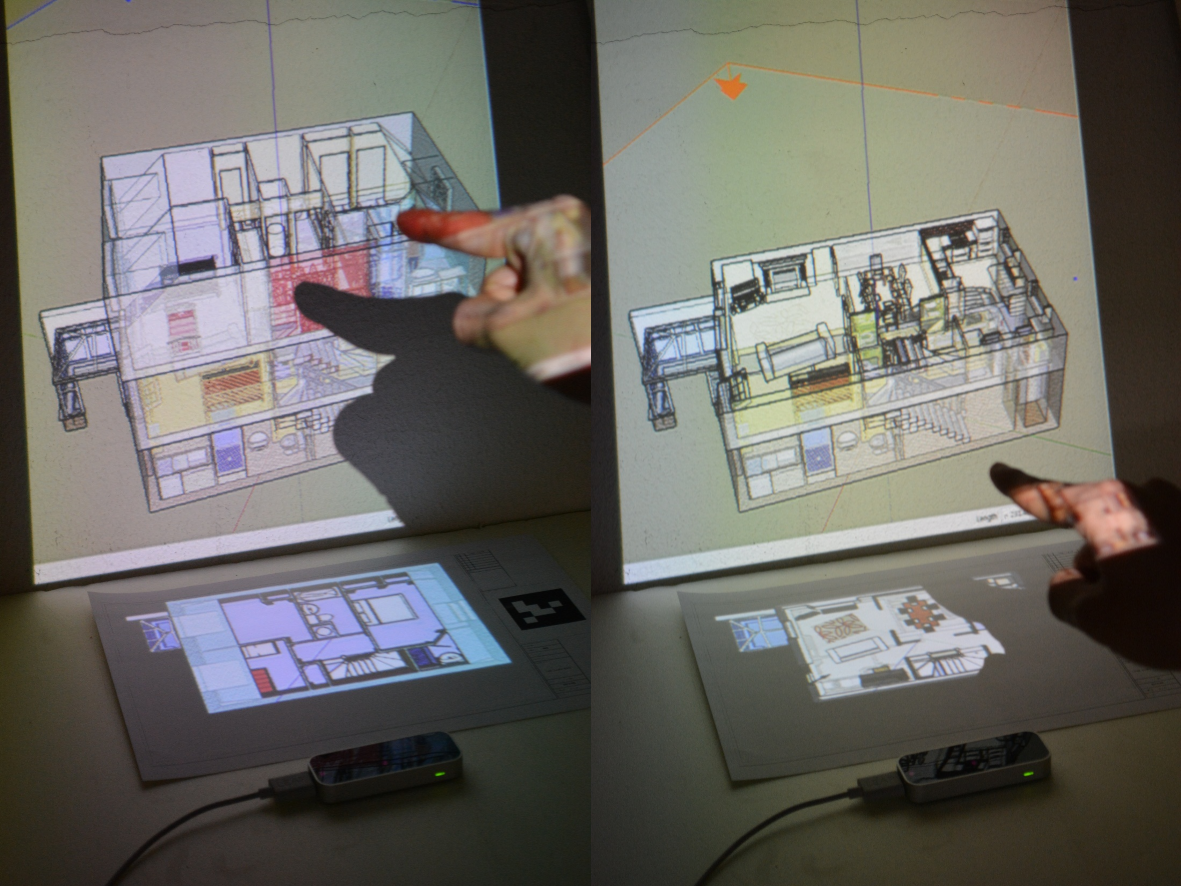
\includegraphics[width=0.7\columnwidth, height=3.6cm]{4-Interaction_Design/query_plane}
\caption{Querying Specific Floor Plan}
\label{fig:layer}
\end{figure}


% \begin{figure*}[t!]
\begin{figure}[h!]
	\centering
        \begin{subfigure}[b]{1.0\columnwidth}
	        \centering
                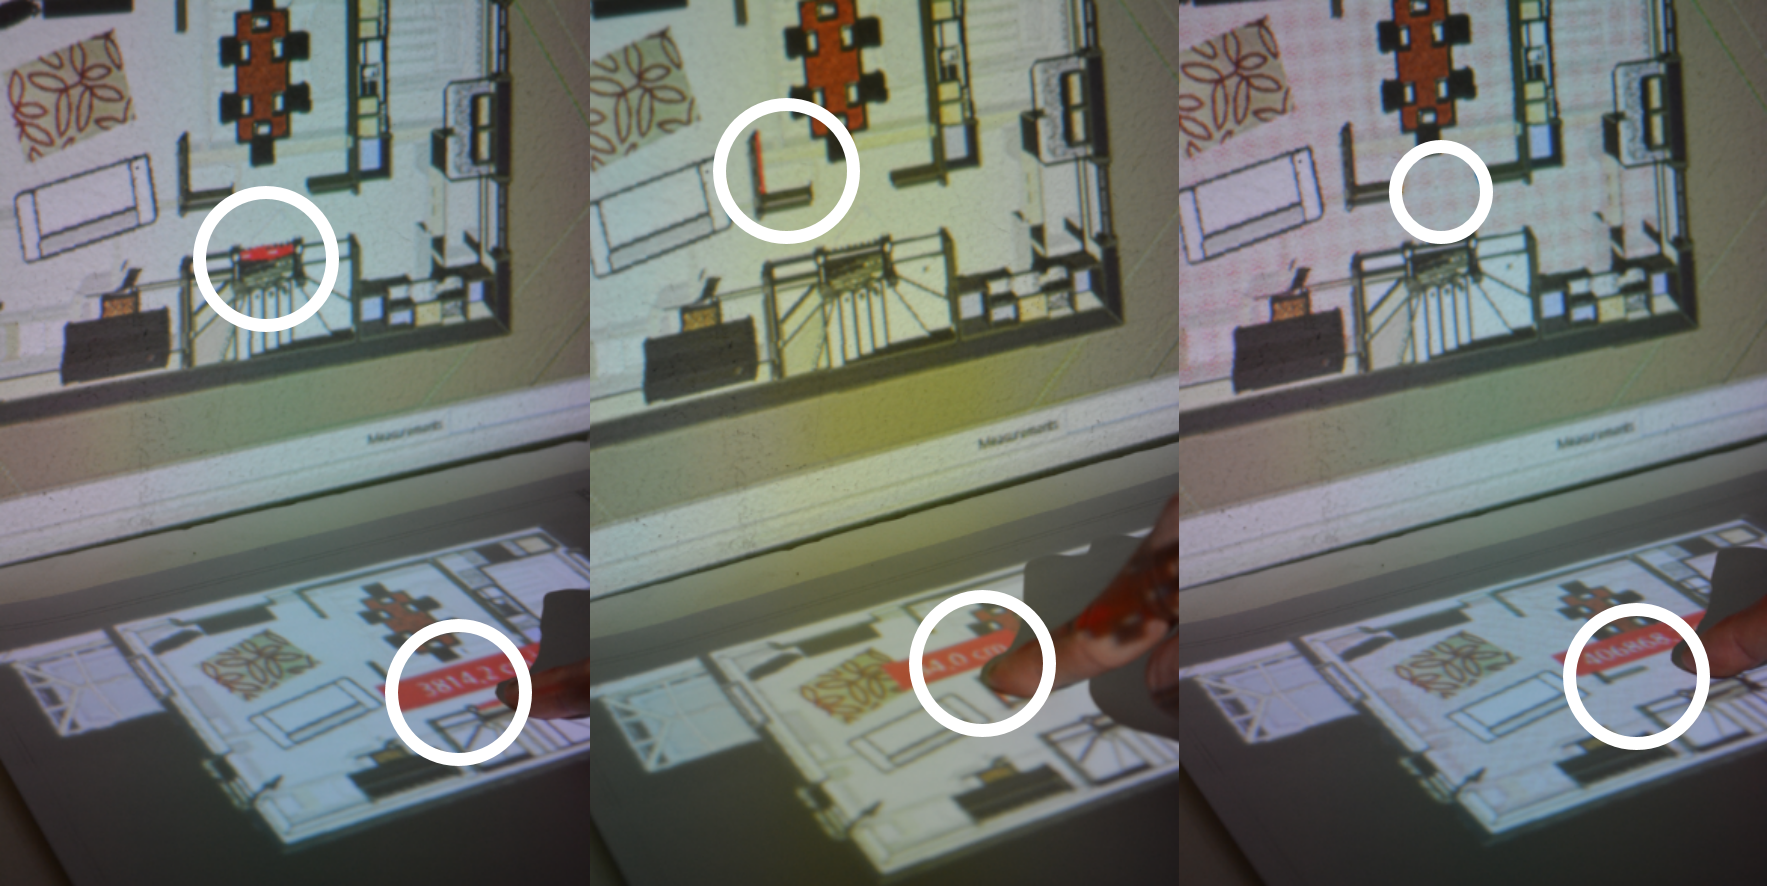
\includegraphics[width=0.9\textwidth, height=3.6cm]{4-Interaction_Design/2d_info}
                \caption{Querying 2D information - length, area, volumn of specific entity}
                \label{fig:2d_info}
        \end{subfigure}%
        \\
        \begin{subfigure}[b]{1.0\columnwidth}
            \centering
            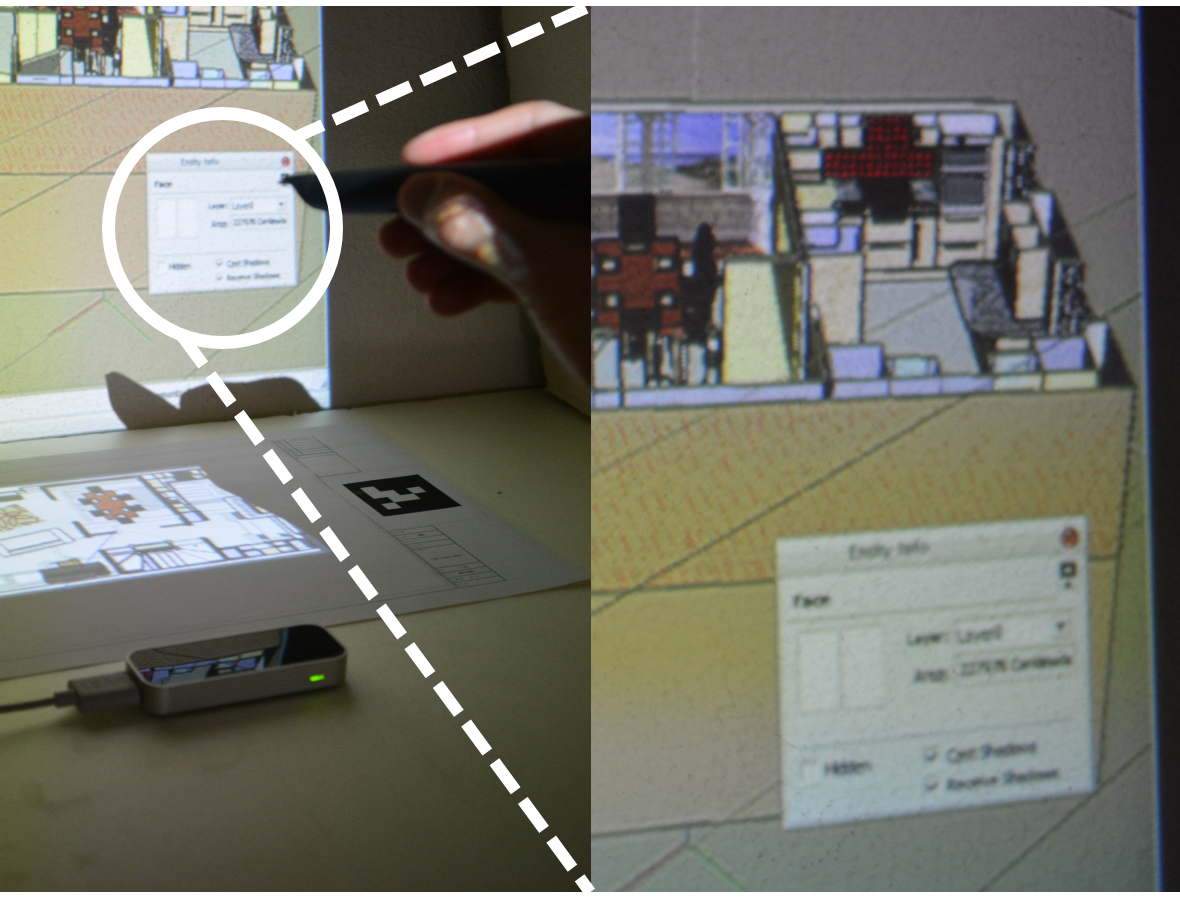
\includegraphics[width=0.7\columnwidth, height=3.6cm]{4-Interaction_Design/3d_info_1}
                \caption{3D information}
                \label{fig:3d_info}
        \end{subfigure}
	\caption{Get Constructional Information by Selecting Entities}
    \label{fig:infor}
% \end{figure*}
\end{figure}


건축 공정 중 특정 평면도의 정보를 접근할 필요가 있다. 이를 위하여 그림 \ref{fig:layer}와 같이 NDH의 한 손가락을 인식하면 평면도 선택 모드로 진입하며, SketchUp의 \textit{Section Plane} 기능을 이용하여 전체 건물 모델에서 특정 평면을 질의하여 Horizontal Screen에 증강하도록 한다. 또한, Mobile Personal Workspace에서는 3D 모드에서 모델 외부를 Drag함으로써 곧바로 Floor plan 선택 모드로 진입하도록 하였다.

%% 번역 원본
% While construction processes, it is necessary to access the information of special floor plans. For this, like Figure \ref{fig:layer}, if a finger of NDH is recognized, a mode of selecting a floor plan is entered. Using the function of \textit{Section Planes} of \textit{SketchUp}, by querying a special plane in all buildings models, the selected floor plan view is expanded onto the horizontal screen. Not only that, but within a \textit{Mobile Personal Workspace}, a model exterior can be dragged in 3D mode to immediately enter Floor Plan Selection Mode.


%% 번역 결과
% During construction processes, it is necessary to access the information of special floor plans. For this purpose, as shown in Figure \ref{fig:layer}, if an NDH finger is recognized, a mode of selecting a floor plan is entered. Using the SketchUp Section Planes function to query a special plane in all building models, the selected floor plan view is expanded onto the horizontal screen.

% In addition, within the mobile personal workspace, a model exterior can be dragged in 3D mode to enter floor plan selection mode immediately.




%%%%%%%%
\subsection{Additional Information Retrieval}

건축 공정 중에 도면의 부가적인 정보를 계산하여야 하는 경우가 빈번하다. 특히 \cite{song_penlight:_2009}에서 제안한 것과 같이 건축 도면에서 부가적인 Dimension 정보를 제공하는 것은 시공 현장에서 유용하게 사용된다. 제안하는 시스템에서는 SketchUp의 Entity 정보를 이용하여 이러한 Dimension 정보를 계산한다. 또한 기존 시스템에서는 2차원 정보만 증강되었던데 반하여 3차원 모델을 in-air에서 터치함으로써 벽면의 넓이나 기둥의 높이 등 3차원 Entity의 Dimension도 제공할 수 있다. 또한, Mobile Personal Workspace에서는 모바일 기기 화면에 있는 컨텐츠를 터치하여 부가적인 정보를 얻을 수 있도록 하였다. 하지만, 손가락으로 터치하는 것이 정밀하지 못하기 때문에 불편하다는 피드백이 많았다. 추후 연구에서는 영역 확대와 같은 기능을 추가하여 인식의 정밀도를 높이는 것이 필요하다.

%% 번역 원본
% Among the construction processes, cases to calculate additional information of blueprints occur often. In particular, like the proposal in \cite{song_penlight:_2009}, to provide additional dimension information in construction blueprints is used frequently at construction work sites. In the proposed system, using entity info of \textit{SketchUp}, this dimension information is calculated. The additional dimension information provided in \cite{song_penlight:_2009} applied it only to the 2D information; on the contrary, by touching 3D models in-air, Port3DAr provides dimensions of 3D entities like area, height, and so on of a wall surface. Furthermore, additional information can be obtained by touching content on a mobile device screen in a Mobile Personal Workspace. However, since touching by hand is not very precise, there was a lot of feedback about ballpoint pens. Further research needs to expand the field and add similar functions to increase the precision of recognition. 

%% 번역 결과
% During construction, the need to calculate additional information regarding blueprints arises often. In particular, as in the proposal in \cite{song_penlight:_2009}, the need to provide additional dimension information in construction blueprints arises frequently at construction work sites. In the proposed system, this dimension information is calculated using SketchUp entity information. The additional dimension information provided in \cite{song_penlight:_2009} applies only to the 2D information; in contrast, Port3DAr provides dimensions of 3D entities, such as area and height, of a wall surface by touching 3D models. Furthermore, additional information can be obtained by touching content on a mobile device screen in a mobile personal workspace. However, since touching by hand is imprecise, there was substantial feedback regarding ballpoint pens. Further research needs to be conducted to expand the field and add similar functions to increase recognition precision.


\subsubsection{2D Information Retrieval}
2차원 정보 제공은 Figure \ref{fig:2d_info}와 같이 도면에 나타난 벽면의 길이(그림 \ref{fig:2d_info} 왼쪽)나 바닥 면(그림 \ref{fig:2d_info} 오른쪽), 가구 등의 부피(그림 \ref{fig:2d_info} 중앙) 등을 도면을 직접 터치함으로써 획득할 수 있다. 이는 해당 건축 도면 상에서 터치된 2차원 좌표를 \textit{SketchUp} 프로그램에 질의하여 \textit{Entity} 정보를 획득하여 보여주게 된다.
%% 번역 원본
% Provision of 2D information can be acquired by touching some parts of a blueprint such as length of a wall surface (see Figure \ref{fig:2d_info} left), floor surface (see Figure \ref{fig:2d_info} right), and bulk of furniture (see Figure \ref{fig:2d_info} center) that are represented on the floor plan like Figure \ref{fig:2d_info}. This makes entity information appear after its acquisition by selecting 2D coordinates touched on the pertinent construction blueprint in the \textit{SketchUp} program.

%% 번역 결과
% 2D information can be acquired by touching parts of a blueprint, such as length of a wall surface (see Figure \ref{fig:2d_info} left) or floor surface (see Figure \ref{fig:2d_info} right) and bulk of furniture (see Figure \ref{fig:2d_info} center), that are represented on the floor plan, as in Figure \ref{fig:2d_info}. This causes entity information to appear after its acquisition by selecting 2D coordinates touched on the pertinent construction blueprint in the SketchUp program.

\subsubsection{3D Information Retrieval}
3차원 정보 제공은 그림 \ref{fig:3d_info}와 같이 3차원 모델의 \textit{entity}를 선택함으로써 정보를 제공받게 된다. Vertical Screen의 3차원 모델을 선택하기 위해서는 Leap Motion 기반의 손가락 인식 기술을 사용하여 Screen Tap 제스처를 이용하여 입력이 제공된다. Mobile Personal Workspace에서는 3D 모드에서 모델을 선택하여 선택된 위치를 SketchUp에 질의하여 정보를 얻게 된다.
%% 번역 원본
% 3-Dimensional Information Retrieval means that, as in Figure \ref{fig:3d_info}, information can be received by selecting a model's entity. To select a 3D model for the Vertical Screen, finger recognition technology based on \textit{Leap Motion} is used with input offered through Screen Tap gestures. In a Mobile Personal Workspace, information can be obtained by selecting a model in 3D mode and querying \textit{SketchUp} for the selected location. 

%% 번역 결과
% 3D information retrieval is accomplished by selecting a model's entity, as in Figure \ref{fig:3d_info}. To select a 3D model for the vertical screen, finger recognition technology based on Leap Motion is used with input offered through screen tap gestures. In a mobile personal workspace, information can be obtained by selecting a model in 3D mode and querying SketchUp for the selected location.

%%%%%%%%
\subsection{On-site Editing}

실제 시공 환경에서는 여러가지 이유로 도면이나 모델의 계획을 벗어나 시공을 수행해야하는 경우들이 발생한다. 현재 시공 환경에서는 건축 정보에 접근과 수정이 어렵기 때문에 이러한 수정 사항들이 도면으로 다시 재반영되어 갱신되지 않는 경우가 많다. 제안하는 시스템에서는 펜이나 터치를 이용하여 기존의 Entity를 선택하고 이를 이동하거나 수정할 수 있도록 하였다. Shared Smart Space 에서는 펜을 이용하고 스케치 인식 기술을 이용하여 수정되어야 하는 내용을 인식하였으며, Mobile Personal Workspace에서는 터치와 Drag를 인식하여 수정사항을 인식하였다.
%% 번역 원본
% In an actual construction environment, there are many reasons why deviation from blueprints or model plans might be necessary to carry out construction. Since it's currently difficult to access or adjust construction information in construction environments, these adjustments are often not reflected or updated in blueprints. In the proposed system, previous entities can be selected and moved or modified using touch or a pen. In a Shared Smart Space, information that must be adjusted using a pen or sketch recognition technology is recognized, and in Mobile Personal Workspace, touch and drag is recognized for adjustments. 

%% 번역 결과
% In an actual construction environment, there are many reasons why deviation from blueprints or model plans might be necessary for construction. Since it is currently difficult to access or adjust construction information in construction environments, these adjustments are often not reflected or updated in blueprints. In the proposed system, previous entities can be selected and moved or modified using touch or a pen. Information that must be adjusted using a pen or sketch recognition technology is recognized in a shared smart space, and touch and drag is recognized for adjustments in a mobile personal workspace.

% \begin{figure*}[t!]
\begin{figure}[h!]
    \centering
        \begin{subfigure}[b]{0.49\columnwidth}
            \centering
                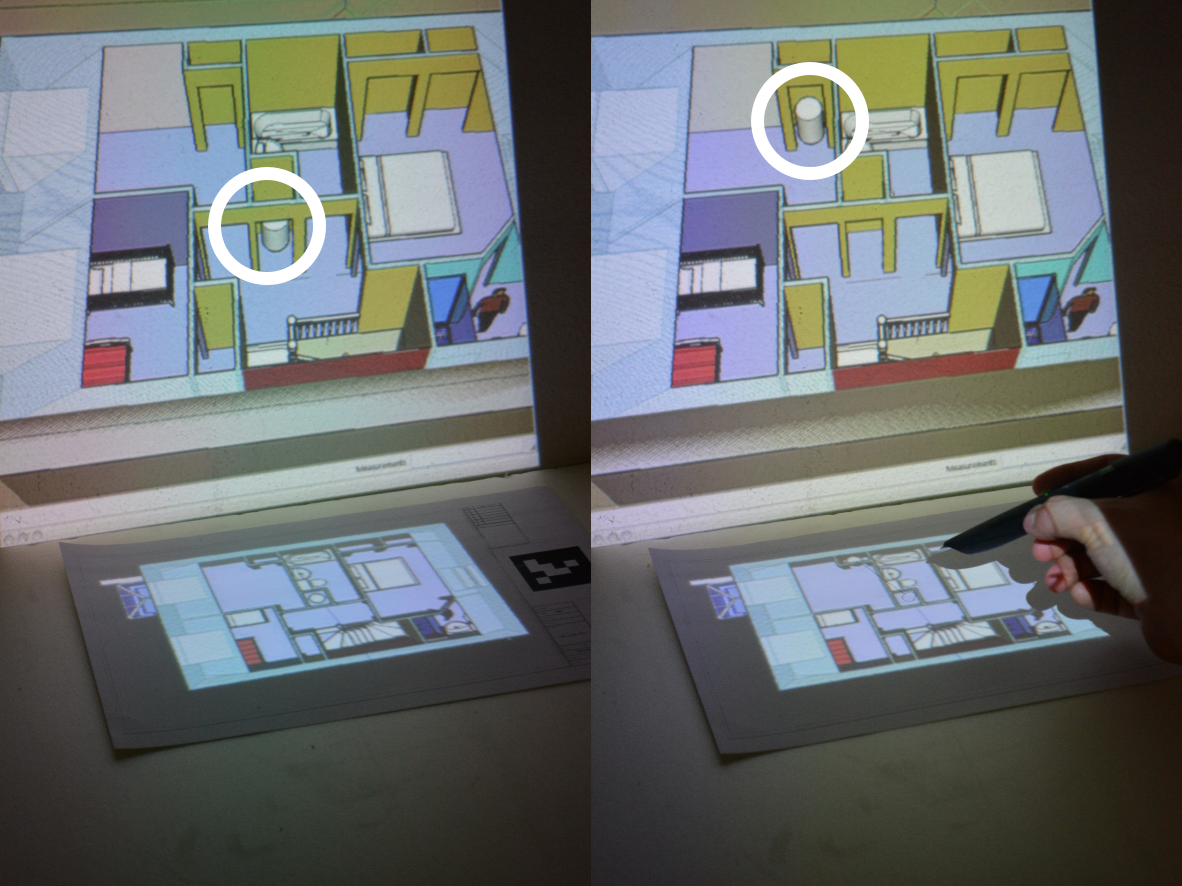
\includegraphics[width=1.0\columnwidth, height=3.6cm]{4-Interaction_Design/2d_move}
                \caption{Modifying 2D Entity using Pen}
                \label{fig:Pen_move}
        \end{subfigure}%
        \hfill
        \begin{subfigure}[b]{0.49\columnwidth}
            \centering
            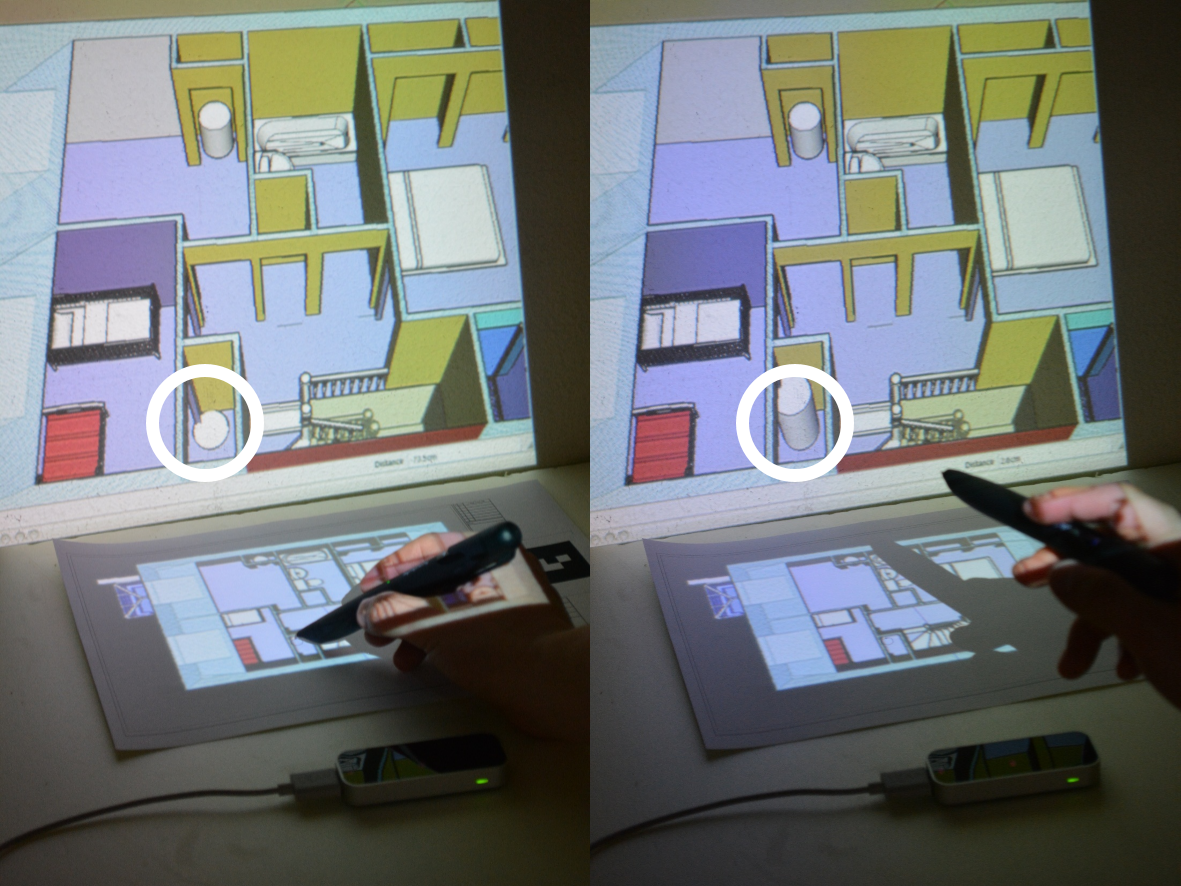
\includegraphics[width=1.0\columnwidth, height=3.6cm]{4-Interaction_Design/3d_note}
                \caption{Modifying 3D Entity in-air}
                \label{fig:Annotation}
        \end{subfigure}
    \caption{On-site Editing using Pen}
    \label{fig:edit}
\end{figure}
% \end{figure*}

\begin{figure*}[b!]
    \centering
        \begin{subfigure}[b]{0.23\textwidth}
            \centering
                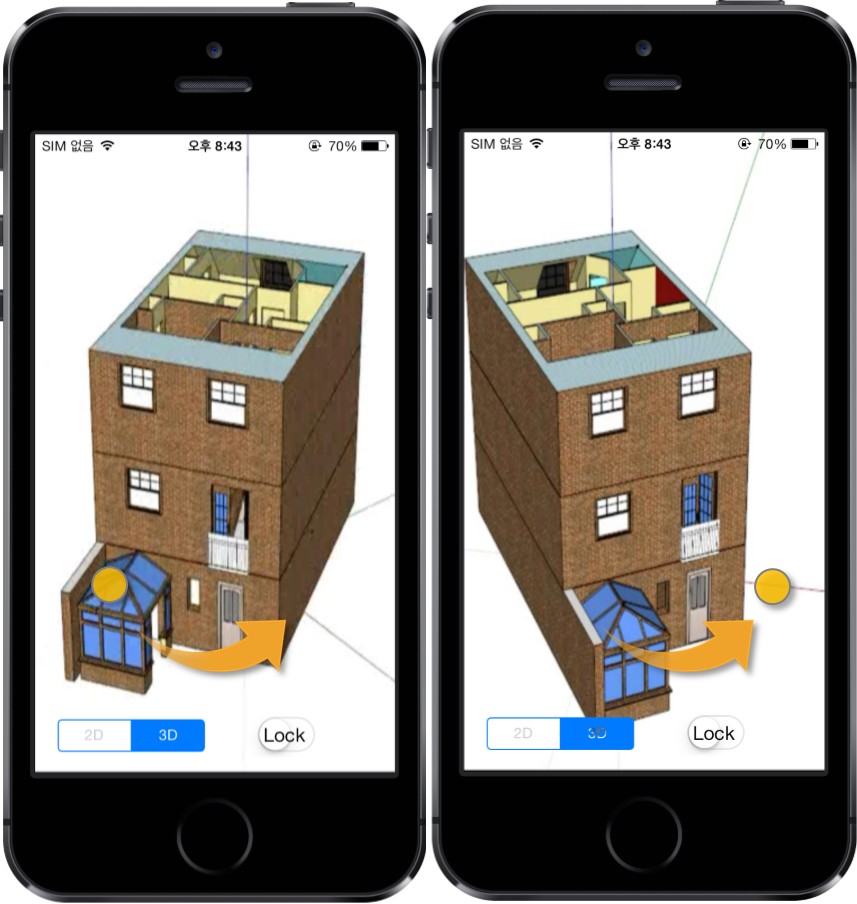
\includegraphics[width=\textwidth, height=3.6cm]{4-Interaction_Design/m_rotate}
                \caption{Rotate by dragging}
                \label{fig:m_rotate}
        \end{subfigure}%
        \hfill
        \begin{subfigure}[b]{0.23\textwidth}
            \centering
            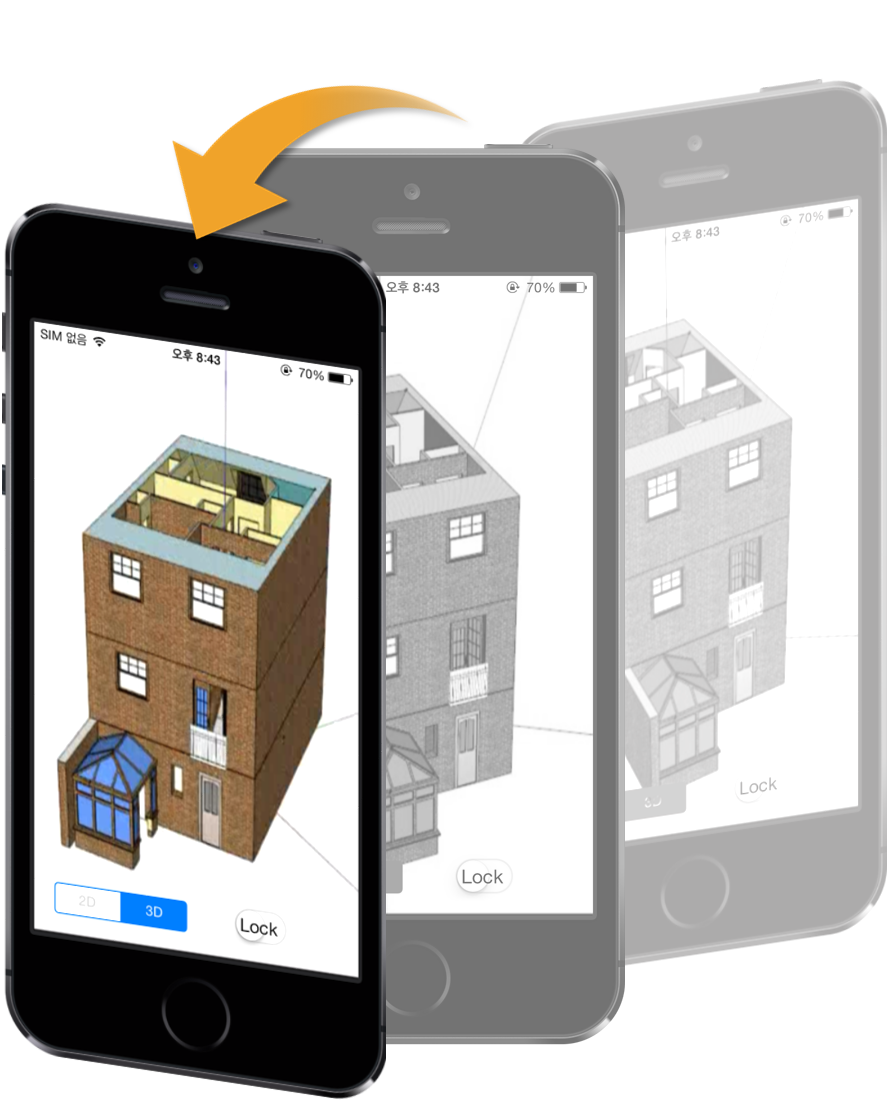
\includegraphics[width=\textwidth, height=4.3cm]{4-Interaction_Design/m_rotate2}
                \caption{Rotate by tilting}
                \label{fig:m_rotate2}
        \end{subfigure}
        \hfill
        \begin{subfigure}[b]{0.23\textwidth}
            \centering
            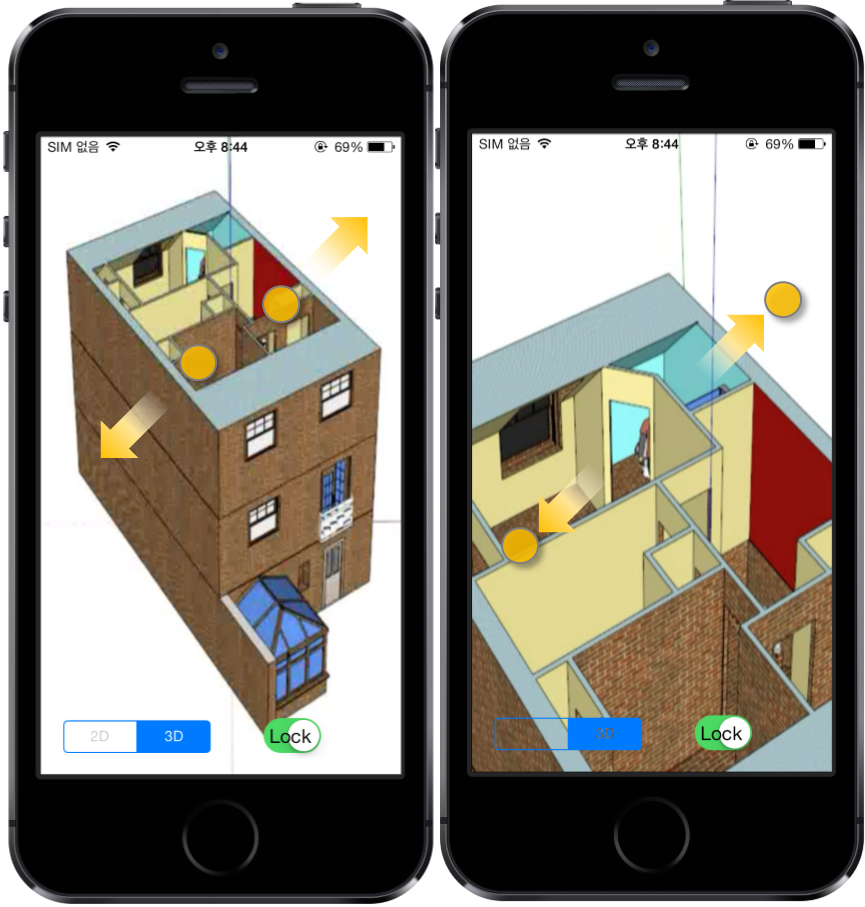
\includegraphics[width=\textwidth, height=3.6cm]{4-Interaction_Design/m_scale}
                \caption{Scale by pinch}
                \label{fig:m_scale}
        \end{subfigure}
        \\
        \begin{subfigure}[b]{0.23\textwidth}
            \centering
                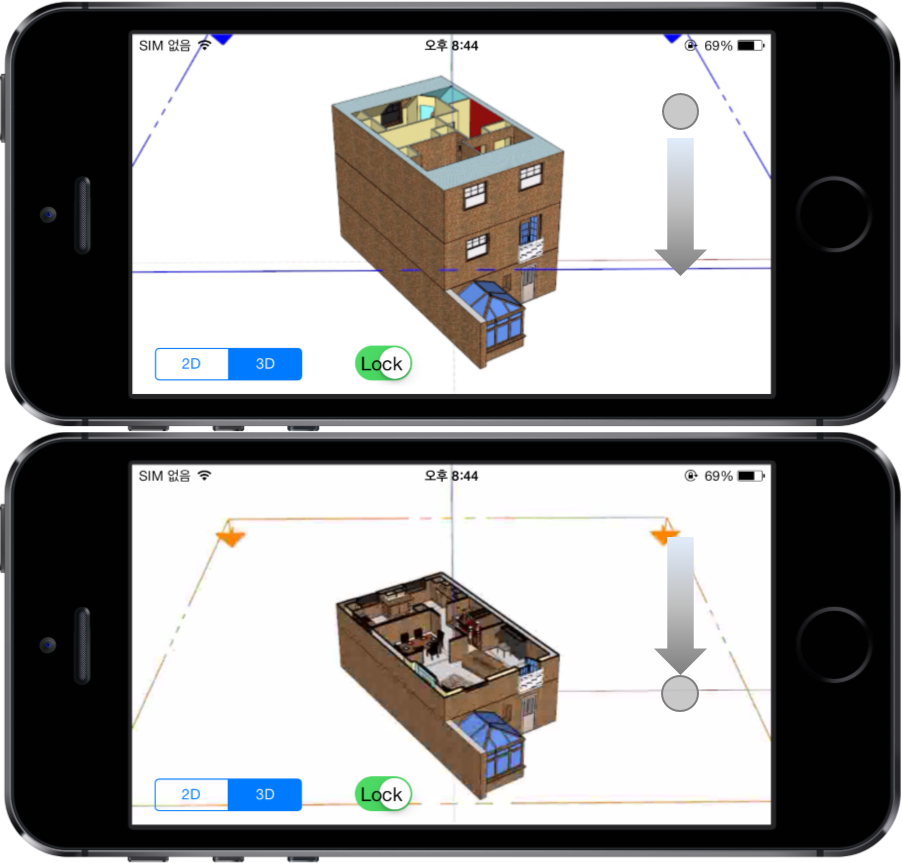
\includegraphics[width=\textwidth, height=3.6cm]{4-Interaction_Design/m_select_plane}
                \caption{Select a floor plane}
                \label{fig:selecting_floor}
        \end{subfigure}%
        \hfill
        \begin{subfigure}[b]{0.23\textwidth}
            \centering
                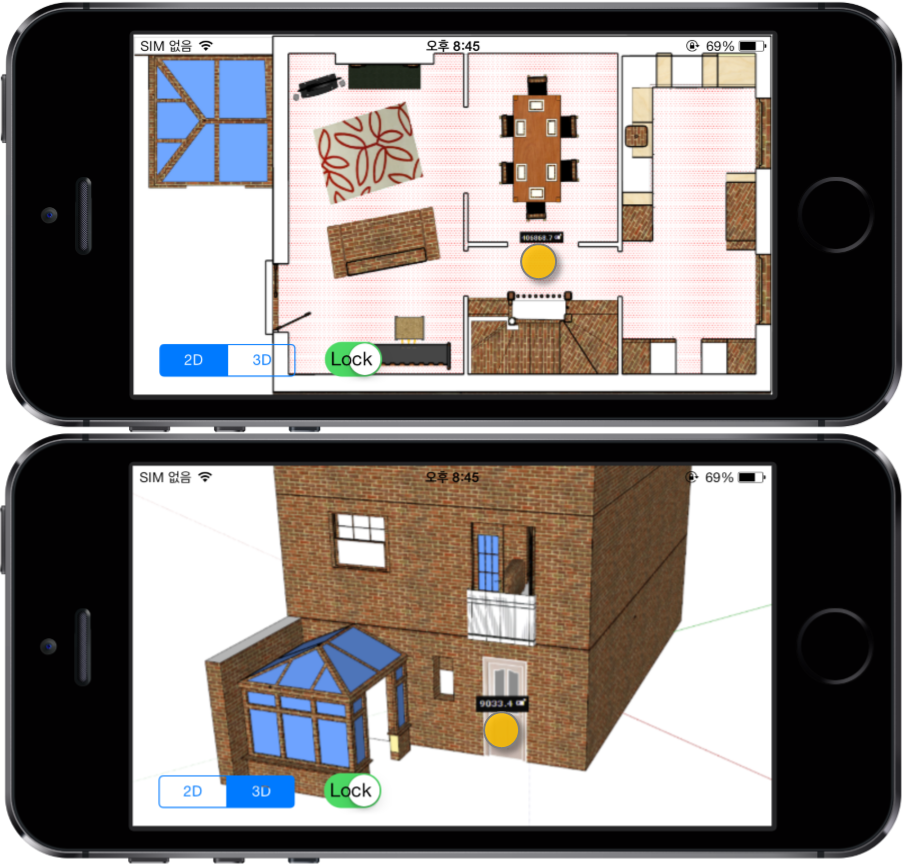
\includegraphics[width=\textwidth, height=3.6cm]{4-Interaction_Design/m_info}
                \caption{Get infor. by touch}
                \label{fig:m_info}
        \end{subfigure}%
        \hfill
        \begin{subfigure}[b]{0.23\textwidth}
            \centering
                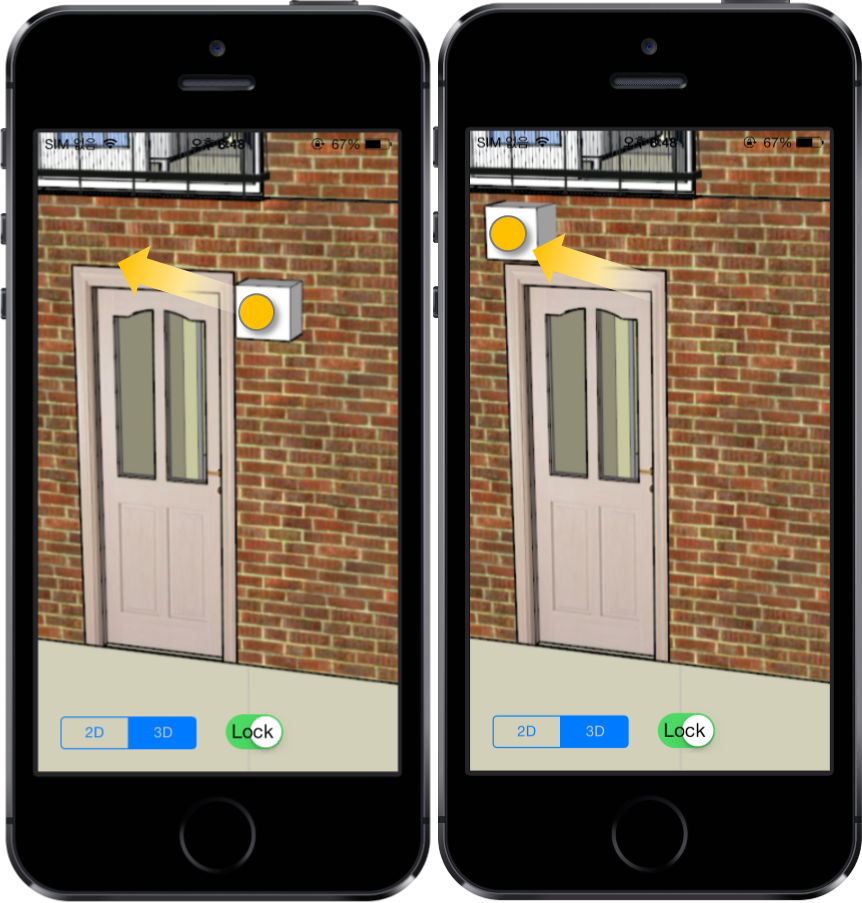
\includegraphics[width=\textwidth, height=3.6cm]{4-Interaction_Design/m_move}
                \caption{Modify on-the-fly}
                \label{fig:m_move}
        \end{subfigure}%
    \caption{Interaction Design for Personal Mobile Workspace}
    \label{fig:pwm_interaction}
\end{figure*}